\chapter{Introduction}
\label{intro}

\begin{itemize}
\item Gov Linkedata, Spatial data and visualizations
\item Evolution of LOD cloud: 2014, 2011, 2007
\item Percentage of geodata on the space
\end{itemize}

\section{Context}
\label{sec:context}

\todo{add 3 figures of LOD evolution: 2007, 2011 and 2014, and explain the differences also regarding geodata. add http://lod-cloud.net/state/}

LOD Cloud 2014 at http://data.dws.informatik.uni-mannheim.de/lodcloud/2014/. The new version altogether contains 570 linked datasets which are connected by 2909 linksets.

\begin{figure}[ht!]
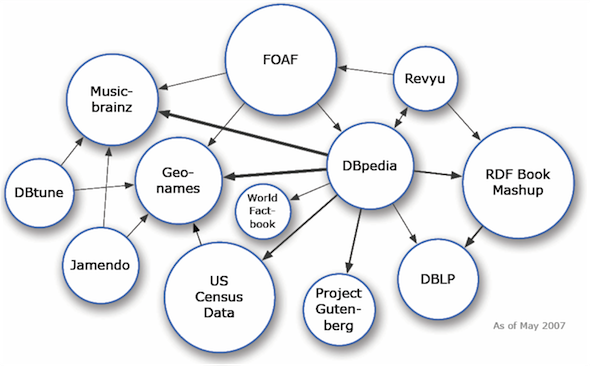
\includegraphics[scale=0.9]{img/lod-cloud2007.png}
\caption{LOD cloud as of May, 2007}
\label{fig:lodcloud2007}
\end{figure}

\begin{figure}[ht!]
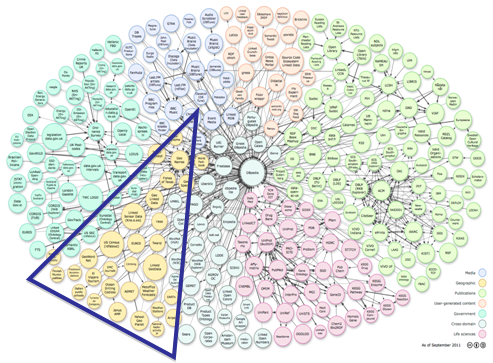
\includegraphics[scale=0.9]{img/lod-diagram-2011.png}
\caption{LOD cloud as of August, 2011}
\label{fig:lodcloud2011}
\end{figure}

\begin{figure}[ht!]
\centering{
\includegraphics[scale=0.1]{img/LODcloud2014.pdf}
\caption{LOD cloud as of April, 2014}
\label{fig:lodcloud2014}
}
\end{figure}





\section{Research Questions}
\label{sec:questions}

\section{Contributions}
\label{sec:contributions}

\section{Thesis Structure}
\label{sec:thesis-structure}